\
\documentclass[usenames,dvipsnames]{beamer}
\mode<presentation>{\usetheme{Warsaw}}
\usepackage{textpos} %package for text positioning

%%%%%%%%%%%%%%%%%%%%%%%%%%%%%%%%%%%%%%%%%%%%%%%%%%%%%%%%%%%%%%%%%%%%%%%%%%%%%%%%%%%%
%Normal Math Packages
\usepackage{amsmath}
\usepackage{amsfonts}
\usepackage{enumerate}
\usepackage{amsmath}
\usepackage{mathtools}
\usepackage{tikz-cd}
\usepackage{ragged2e}
\usepackage{mathrsfs}
%%%%%%%%%%%%%%%%%%%%%%%%%%%%%%%%%%%%%%%%%%%%%%%%%%%%%%%%%%%%%%%%%%%%%%%%%%%%%%%%%%%%

%%%%%%%%%%%%%%%%%%%%%%%%%%%%%%%%%%%%%%%%%%%%%%%%%%%%%%%%%%%%%%%%%%%%%%%%%%%%%%%%%%%%
%Created Commands
\theoremstyle{definition}
\newtheorem*{remark}{Remark}
\newtheorem*{question}{Question}
%\newtheorem*{definition}{Definition}
%\newtheorem*{definitions}{Definitions}

\theoremstyle{theorem}
\newtheorem*{proposition}{Proposition}
\newtheorem*{axiom}{Axiom}

\newcommand{\R}{\mathbb{R}}
\newcommand{\Q}{\mathbb{Q}}
\newcommand{\F}{\mathbb{F}}
\newcommand{\A}{\mathcal{A}}
\newcommand{\N}{\mathbb{N}}
\newcommand{\C}{\mathbb{C}}
\newcommand{\opO}{\mathcal{O}}
\newcommand{\states}{\mathcal{S}}
%%%%%%%%%%%%%%%%%%%%%%%%%%%%%%%%%%%%%%%%%%%%%%%%%%%%%%%%%%%%%%%%%%%%%%%%%%%%%%%%%%%%


%%%%%%%%%%%%%%%%%%%%%%%%%%%%%%%%%%%%%%%%%%%%%%%%%%%%%%%%%%%%%%%%%%%%%%%%%%%%%%%%%%%%
%Stuff to make things look good
% Color modification
\setbeamercolor{structure}{fg=green!30!black}% to modify  immediately all palettes
\setbeamercolor{title}{fg=white}
\setbeamercolor{title in head/foot}{fg=yellow}

%Size Modification
\setbeamerfont{frametitle}{size=\small}

% position the logo
\addtobeamertemplate{frametitle}{}{%
\begin{textblock*}{1cm}(\textwidth,-.5cm)

\includegraphics[height=.9cm,width=.9cm,keepaspectratio]{csu.png}
\end{textblock*}}

% Text Positioning
\usepackage[absolute,overlay]{textpos}
%%%%%%%%%%%%%%%%%%%%%%%%%%%%%%%%%%%%%%%%%%%%%%%%%%%%%%%%%%%%%%%%%%%%%%%%%%%%%%%%%%%%

%Font
%\fontfamily{cmr}\selectfont
\usefonttheme{serif}

%Colors and stuf
\usepackage{color, soul, xcolor} % Colored text and highlighting, respectively
\usepackage{tikz-cd} % For commutative diagrams

%% preamble
\title{Differential and Symplectic Geometry}
\subtitle{Clayton Shonkwiler and Patrick Shipman}

\begin{document}

%%Title Frame
{
\setbeamertemplate{headline}{}
\addtobeamertemplate{frametitle}{\vspace*{-0.9\baselineskip}}{}
\begin{frame}
\titlepage
\end{frame}
}


%%%%%%%%%%%%%%%%%%%%%%%%%%%%%%%%%%%%%%%%%%%%%%%%%%%%%%%%%%%%%%%%%%%%%%%%%%%%%%%
%%%%%%%%%%%%%%%%%%%%%%%%%%%%%%%%%%%%%%%%%%%%%%%%%%%%%%%%%%%%%%%%%%%%%%%%%%%%%%%
    
    \begin{frame}{Hey it's this guy}
        \begin{figure}
            \centering
            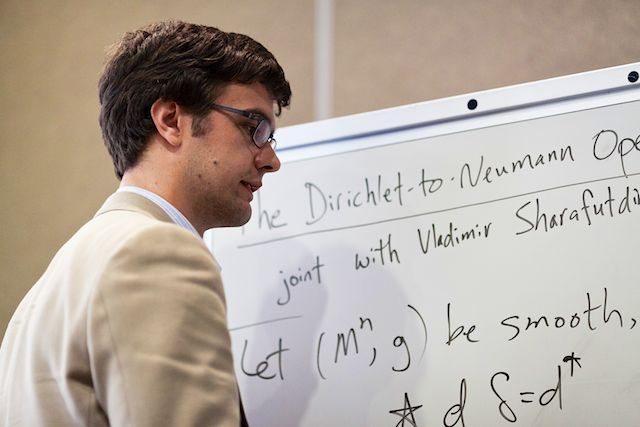
\includegraphics[width=.8\textwidth]{clay.jpg}
        \end{figure}
    \end{frame}
    
    
    \begin{frame}{Interests}
        \begin{itemize}
            \item Differential and symplectic geometry
            \item Applications to synthetic chemistry, polymer physics, and frame theory
            \item Polygon spaces and geometric probability/measure
        \end{itemize}
    \end{frame}

    \begin{frame}{Art}
    \begin{center}
        See: Shonkwiler.org
        \begin{figure}
            \centering
            
\includegraphics[width=.6\textwidth]{33700724514_35273ae7ca_b.jpg}
        \end{figure}
        \end{center}
    \end{frame}
    
        \begin{frame}{Art}
    \begin{center}
        See: Shonkwiler.org
        \begin{figure}
            \centering
            
\includegraphics[width=.6\textwidth]{download.png}
        \end{figure}
        \end{center}
    \end{frame}
    
    \begin{frame}{Art}
    \begin{center}
        See: Shonkwiler.org
        \begin{figure}
            \centering
            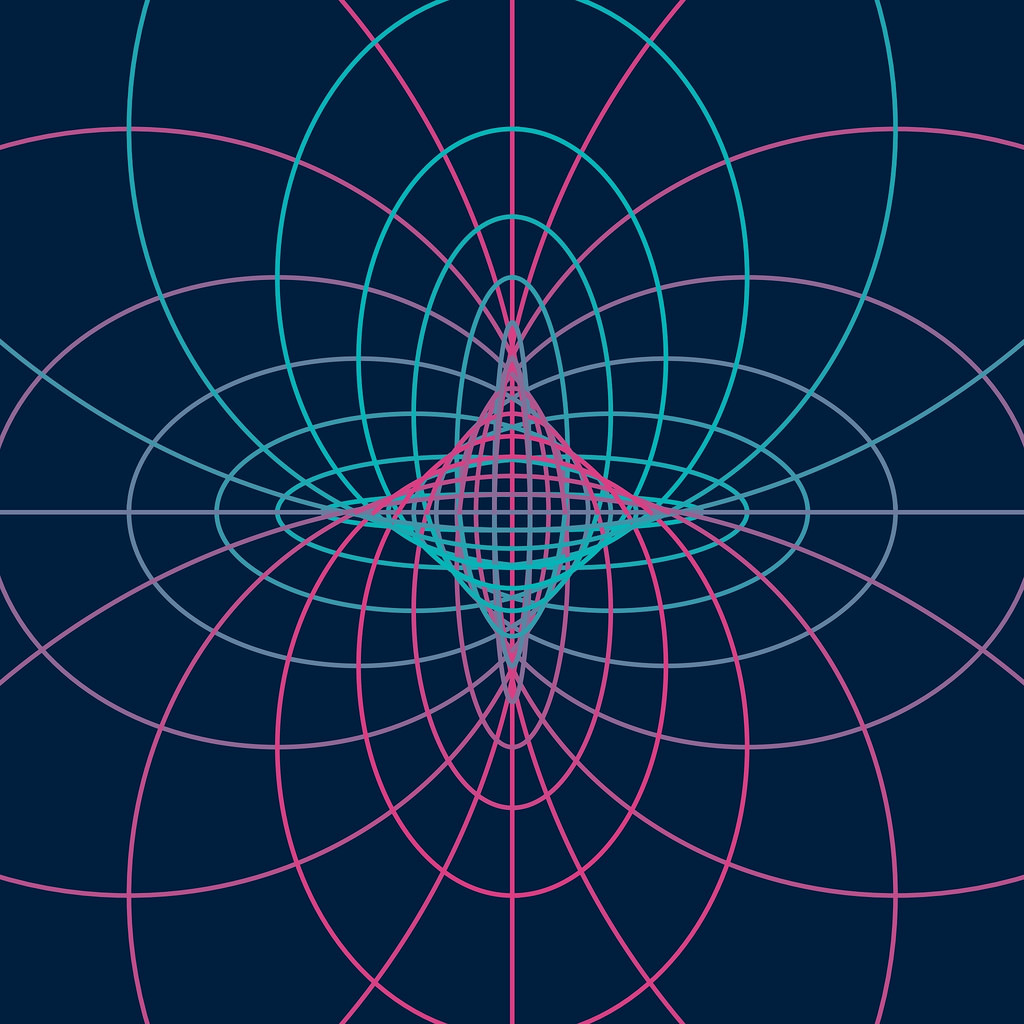
\includegraphics[width=.6\textwidth]{37205108544_283ce78bbf_b.jpg}
        \end{figure}
        \end{center}
    \end{frame}
    
        \begin{frame}{Art}
    \begin{center}
        See: Shonkwiler.org
        \begin{figure}
            \centering
            
\includegraphics[width=.6\textwidth]{platonic5.png}
        \end{figure}
        \end{center}
    \end{frame}
    
    \begin{frame}{The Pillow Problem}
    \begin{itemize}
        \item Lewis Carroll asked the question, "Three points are taken at random on an infinite plane. Find the chance of their being the vertices of an obtuse-angled triangle."
        \item It turns out there is a nice way to think about this by realizing the correspondence to a probability distribution on a Grassmann manifold of 2-planes in 3-space.
    \end{itemize}

    \end{frame}
        
\end{document}